% ======================================================================
% DIAPOSITIVAS DE RESPALDO (no se numeran con la charla principal)
% ======================================================================
\section{Respaldo}
\bloque{RESPALDO}

% ---------------------------------------------------------------- R0
\begin{frame}[plain]
  \begin{tikzpicture}[remember picture, overlay]
    \fill[itedaTeal] (current page.south west) rectangle (current page.north east);
    \node[text=white, font=\fontsize{26}{30}\selectfont\bfseries] at (current page.center)
      {Respaldo};
    \node[text=white!80, font=\small, anchor=north] at ([yshift=-0.7cm]current page.center)
      {cálculos, figuras adicionales de la tesis y material de referencia};
  \end{tikzpicture}
\end{frame}

% ---------------------------------------------------------------- R1
\begin{frame}{Respaldo: las cuentas de las escalas de energía y flujo}
  \begin{columns}[T,onlytextwidth]
    \column{0.49\textwidth}
      \small
      \textbf{Energía}
      \[ 1\,\mathrm{eV}=1{,}602\times10^{-19}\,\mathrm{J}
         \;\Rightarrow\; 10^{20}\,\mathrm{eV}=16{,}0\,\mathrm{J} \]
      \[ \tfrac12(0{,}145\,\mathrm{kg})(25\,\mathrm{m/s})^2=45{,}3\,\mathrm{J}
         \approx 2{,}8\times10^{20}\,\mathrm{eV} \]
      \textbf{Centro de masa} (blanco en reposo, $E\gg m$)
      \[ \sqrt{s}=\sqrt{2Em_pc^2}:\quad
         \begin{cases}10^{17}\,\mathrm{eV}\to 13{,}7\,\mathrm{TeV}\\
         10^{20}\,\mathrm{eV}\to 433\,\mathrm{TeV}\end{cases} \]
    \column{0.48\textwidth}
      \small
      \textbf{Tasa en Auger}
      \[ \frac{\approx5\times10^4\ \text{eventos}}{19\ \text{años}\times3000\,\mathrm{km^2}}
         \approx 0{,}9\ \mathrm{km^{-2}\,año^{-1}}\quad(E>8\,\mathrm{EeV}) \]
      Exposición acumulada: $\approx1{,}2\times10^{5}$\,km$^2$\,sr\,año (ICRC 2025).\\[6pt]
      \textbf{Cherenkov}
      \[ \frac{d^2N}{dx\,d\lambda}=\frac{2\pi\alpha}{\lambda^2}
         \Big(1-\frac{1}{\beta^2n^2}\Big) \]
      {\footnotesize En agua, entre 300 y 600\,nm: $\approx330$ fotones/cm para
      $\beta\to1$. Umbral $\gamma=1{,}52$: $T_e=0{,}26$\,MeV, $T_\mu=55$\,MeV.}
  \end{columns}
\end{frame}

% ---------------------------------------------------------------- R2
\begin{frame}{Respaldo: el modelo analítico de la asimetría (tesis, Cap.~3)}
  \begin{columns}[c,onlytextwidth]
    \column{0.62\textwidth}
      \centering
      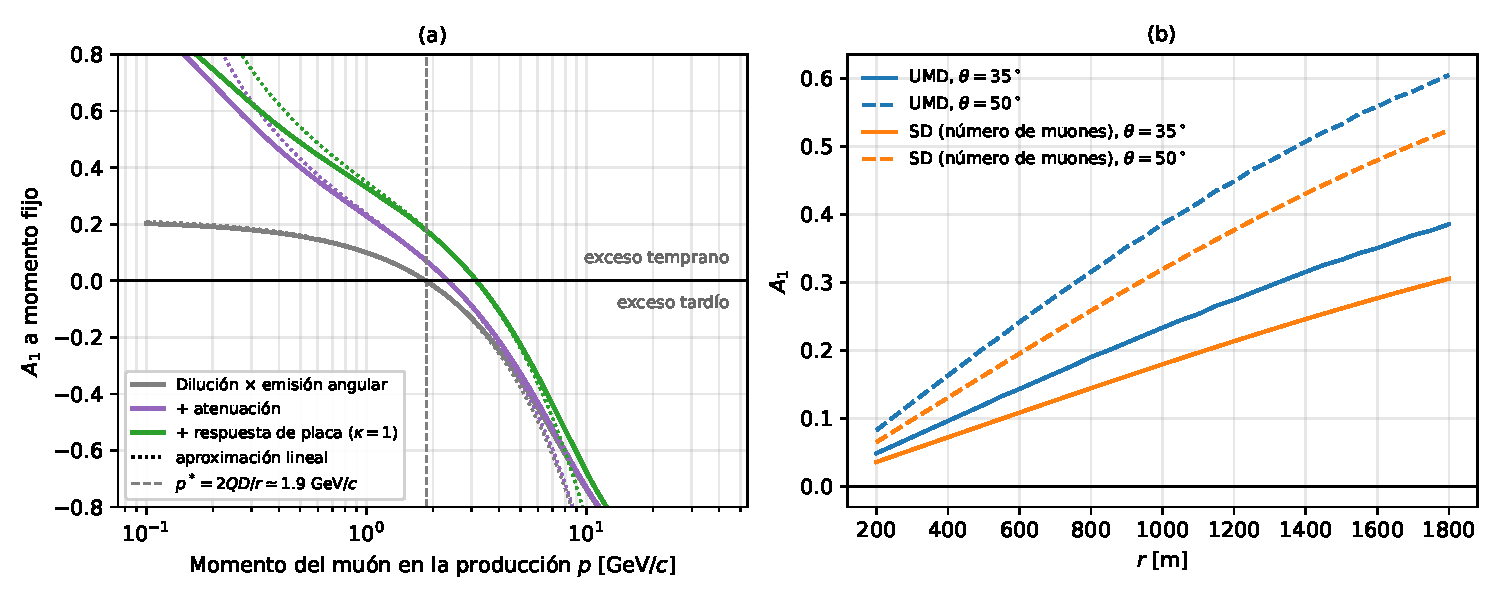
\includegraphics[width=\linewidth]{tesis/modelo_juguete.pdf}
    \column{0.35\textwidth}
      \small
      Reúne dilución, atenuación, respuesta del detector y divergencia
      cinemática. Predice $A_1>0$ en el UMD y el SD, creciente con $r$ y $\theta$.
      \begin{clave}
        La divergencia favorece la región tardía sólo para
        $p > p^*\simeq 2QD/r$: esos muones escasean lejos del núcleo.
      \end{clave}
  \end{columns}
\end{frame}

% ---------------------------------------------------------------- R3
\begin{frame}{Respaldo: sesgo direccional en la reconstrucción de $N_\mu$}
  \begin{columns}[c,onlytextwidth]
    \column{0.55\textwidth}
      \centering
      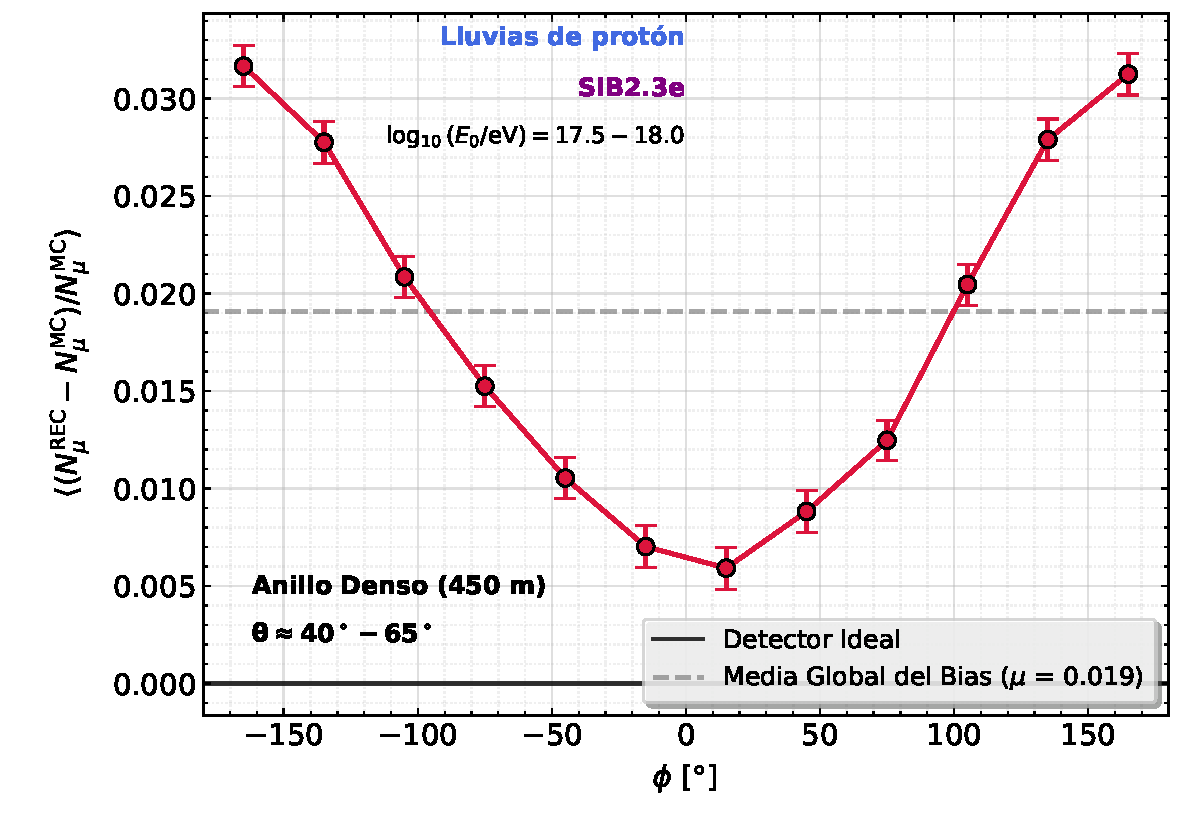
\includegraphics[width=\linewidth]{tesis/directional_bias.pdf}
    \column{0.42\textwidth}
      \small
      El sobreconteo medio es mayor del lado \textbf{tardío}, donde la
      densidad es menor: el error de reconstrucción depende del azimut.
      \begin{clave}
        Un modelo que inyecta los residuos empíricos por azimut reproduce la
        amplitud reconstruida hasta $\theta\approx35^\circ$ y explica la mitad
        o dos tercios de la pérdida más arriba.
      \end{clave}
  \end{columns}
  \credito{Anillo Denso, protones, SIBYLL 2.3e. Tesis, Cap.~5}
\end{frame}

% ---------------------------------------------------------------- R4
\begin{frame}{Respaldo: ¿quiénes quedan afuera de la selección?}
  \centering
  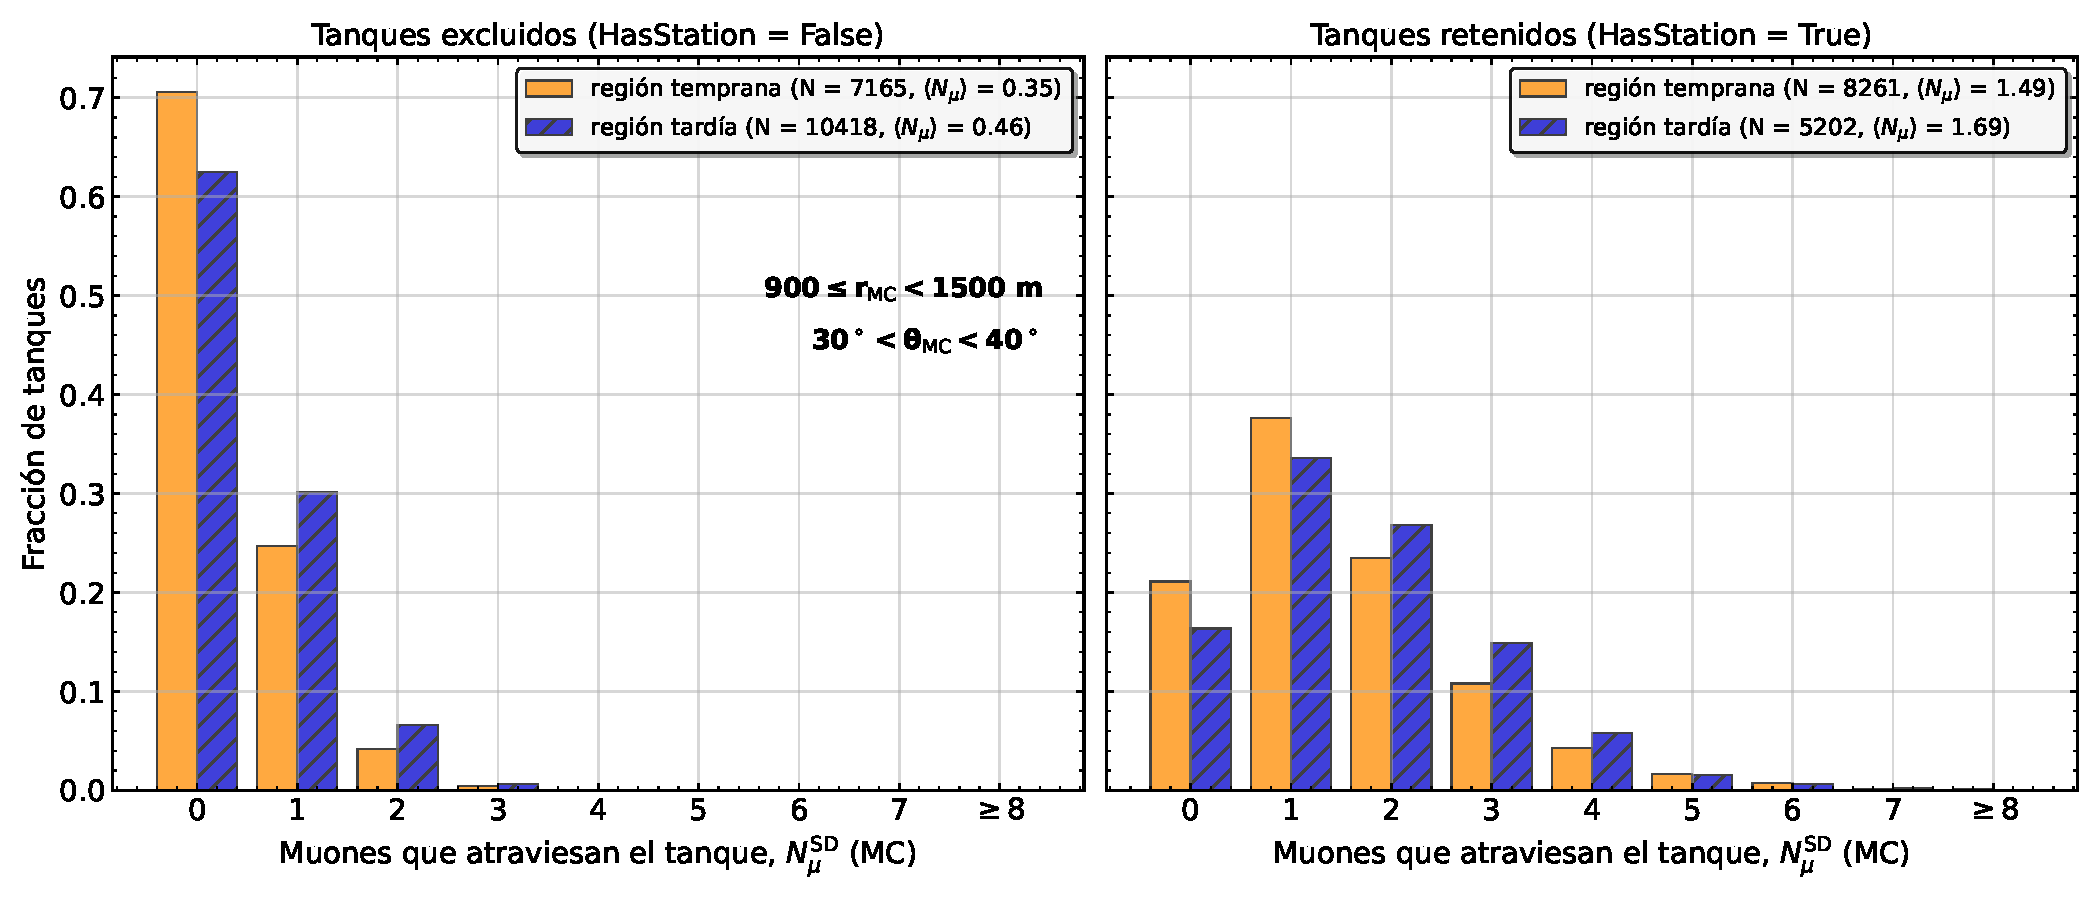
\includegraphics[width=0.8\linewidth]{tesis/SD_Muones_Tanques_Excluidos.pdf}\\[4pt]
  \begin{columns}[T,onlytextwidth]
    \column{0.48\textwidth}
      \footnotesize Tanques excluidos con $\le1$ muón: 95\% (tempranos) y
      93\% (tardíos); media 0,35 y 0,46.
    \column{0.48\textwidth}
      \footnotesize Retenidos: 1,49 (tempranos) y 1,69 (tardíos) muones, aunque
      la densidad incidente es mayor del lado temprano.
  \end{columns}
  \credito{$900\le r<1500$\,m, $30^\circ$--$40^\circ$, geometría MC. Tesis, Cap.~6}
\end{frame}

% ---------------------------------------------------------------- R5
\begin{frame}{Respaldo: el desglose de la señal del SD}
  \begin{columns}[c,onlytextwidth]
    \column{0.58\textwidth}
      \centering
      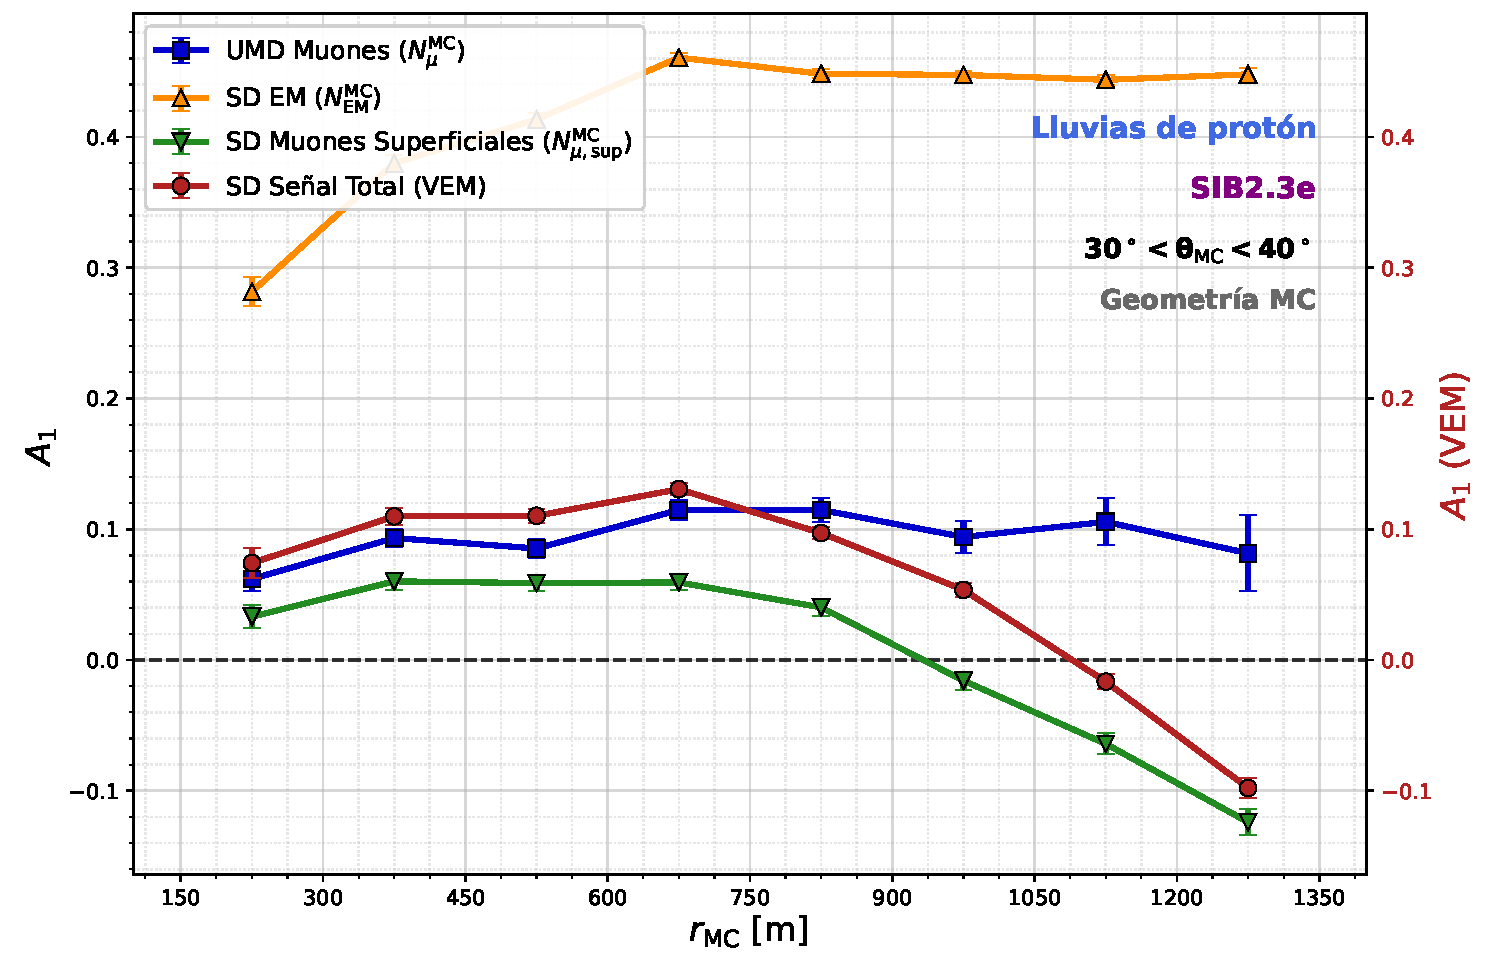
\includegraphics[width=\linewidth]{tesis/SD_Desglose_Componentes_vs_UMD.pdf}
    \column{0.39\textwidth}
      \small
      La componente electromagnética del SD es fuertemente positiva; los
      muones del SD, calculados sobre estaciones seleccionadas, se invierten
      lejos del núcleo y arrastran a la señal total.
      \begin{clave}
        Aun sin selección, entre 150 y 900\,m el UMD supera a los muones del SD
        en 0,03--0,06 (excluye cero al 95\%): diferencia abierta.
      \end{clave}
  \end{columns}
  \credito{Protones, $30^\circ$--$40^\circ$, geometría MC. Tesis, Cap.~6}
\end{frame}

% ---------------------------------------------------------------- R6
\begin{frame}{Respaldo: $A_1(r,\theta)$ en el arreglo de 750\,m}
  \begin{columns}[T,onlytextwidth]
    \column{0.49\textwidth}
      \centering
      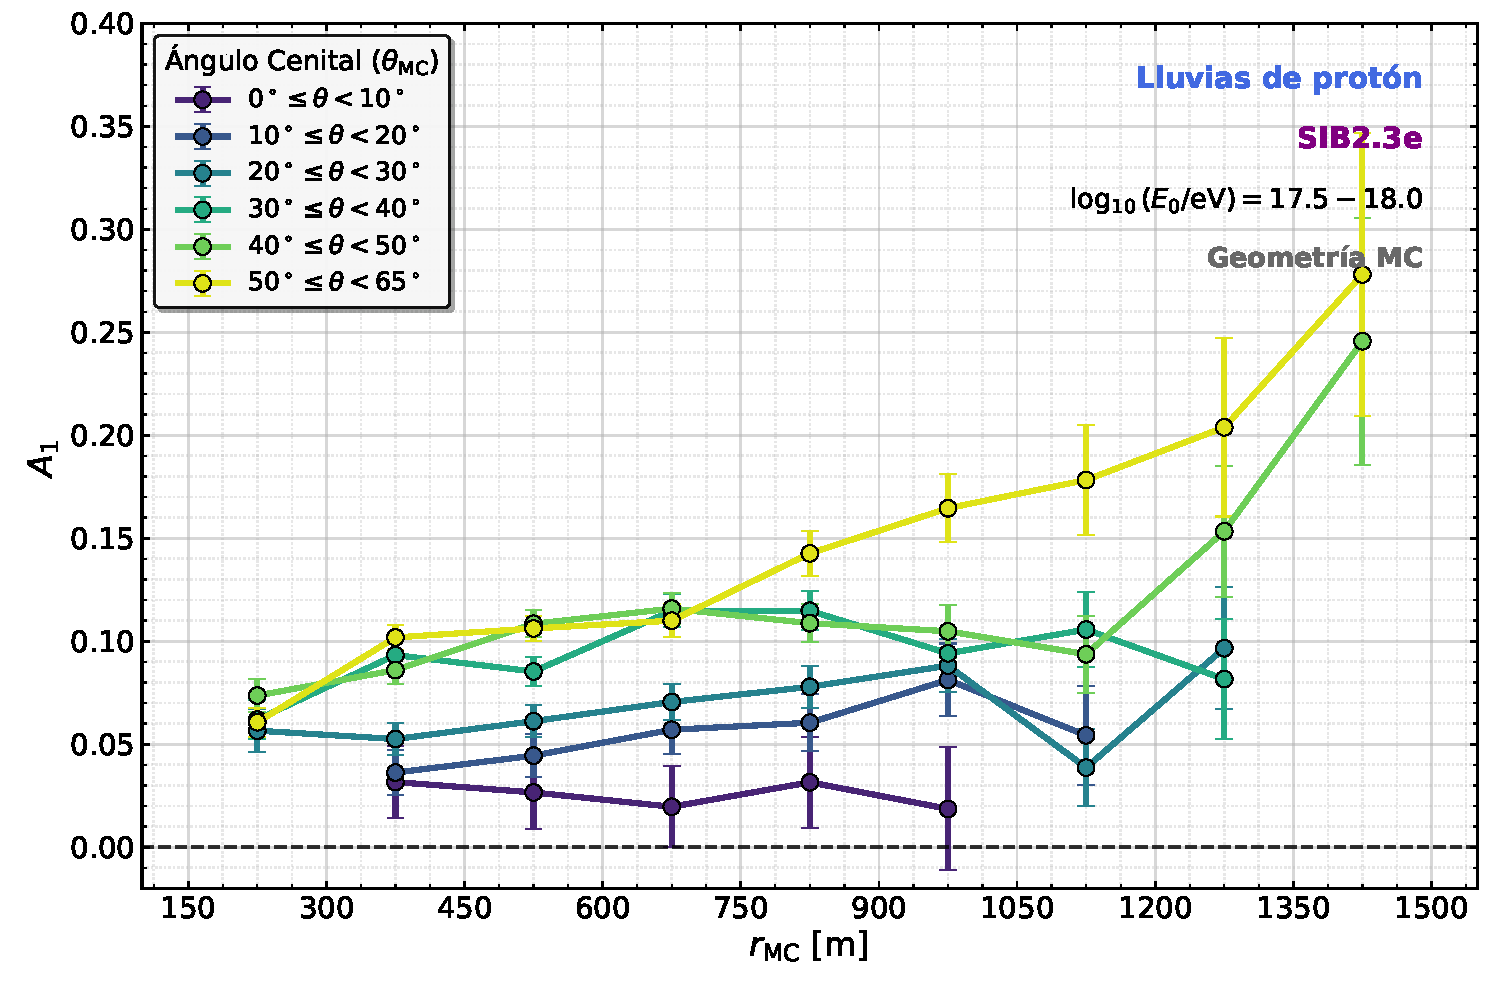
\includegraphics[width=\linewidth]{tesis/Global_A1_vs_R_Theta_MC.pdf}\\
      {\footnotesize Geometría MC: crece con $r$ y $\theta$.}
    \column{0.49\textwidth}
      \centering
      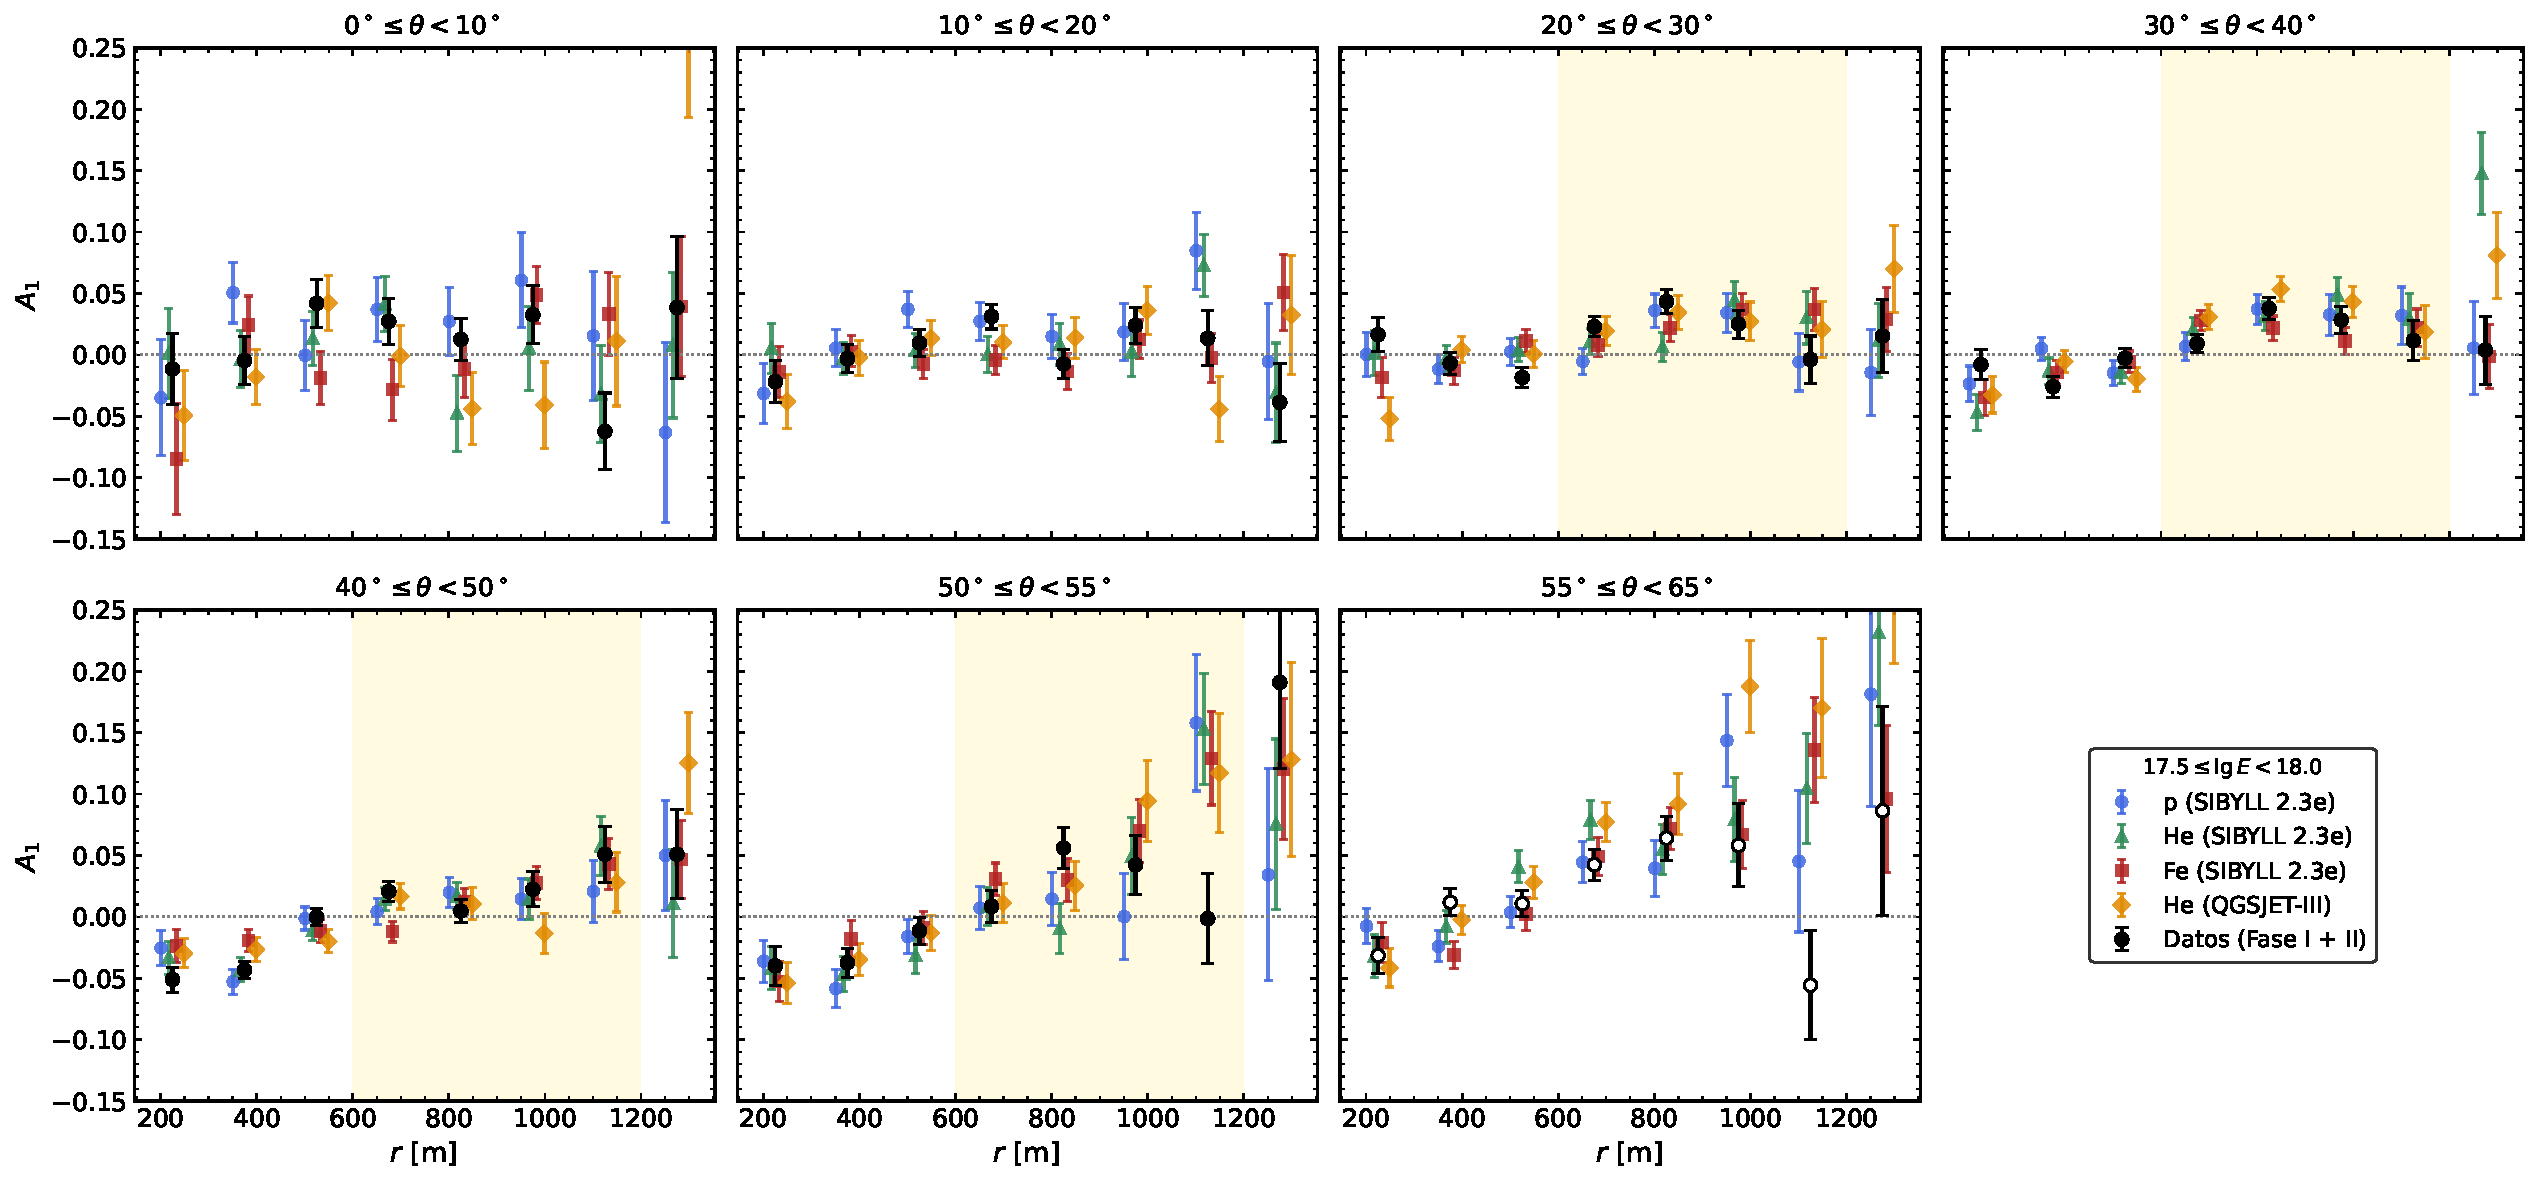
\includegraphics[width=\linewidth]{tesis/cap7_A1_vs_r_datos_vs_mc.pdf}\\
      {\footnotesize Datos (negro) frente a simulaciones reconstruidas,
      $17{,}5\le\lg E<18$.}
  \end{columns}
  \credito{Tesis, Cap.~6. Datos de campo: preliminar}
\end{frame}
